A Tabela \ref{tab:tempos_shell} apresenta os tempos de execução, em segundos, obtidos para o Shell Sort nos seis tamanhos de instância exigidos pelo trabalho, para cada um dos três tipos de entrada testados.

\begin{table}[htbp]
    \centering
    \begin{tabular}{|l|r|r|r|r|r|r|}
        \hline
         & 10 & 100 & 1.000 & 10.000 & 100.000 & 1.000.000 \\
        \hline
        Crescente & 0,000003 & 0,000001 & 0,000005 & 0,000065 & 0,000690 & 0,008251 \\
        \hline
        Decrescente & 0,000002 & 0,000002 & 0,000009 & 0,000083 & 0,001082 & 0,011790 \\
        \hline
        Random & 0,000003 & 0,000004 & 0,000052 & 0,000655 & 0,008226 & 0,106033 \\
        \hline
    \end{tabular}
    \caption{Tempo de execução (em segundos) do Shell Sort por tamanho e tipo de instância}
    \label{tab:tempos_shell}
\end{table}


O Gráfico \ref{fig:grafico_shell} apresenta esses mesmos dados em escala linear. Diferentemente dos três algoritmos anteriores, mesmo a entrada decrescente permanece com tempo de execução muito baixo -- como discutido na análise de complexidade, uma entrada totalmente decrescente não é o pior caso teórico da sequência de gaps utilizada. Para 1.000.000 de elementos, os tempos foram de 0,008 s (crescente), 0,012 s (decrescente) e 0,106 s (randômica).

\begin{figure}[htbp]
    \centering
    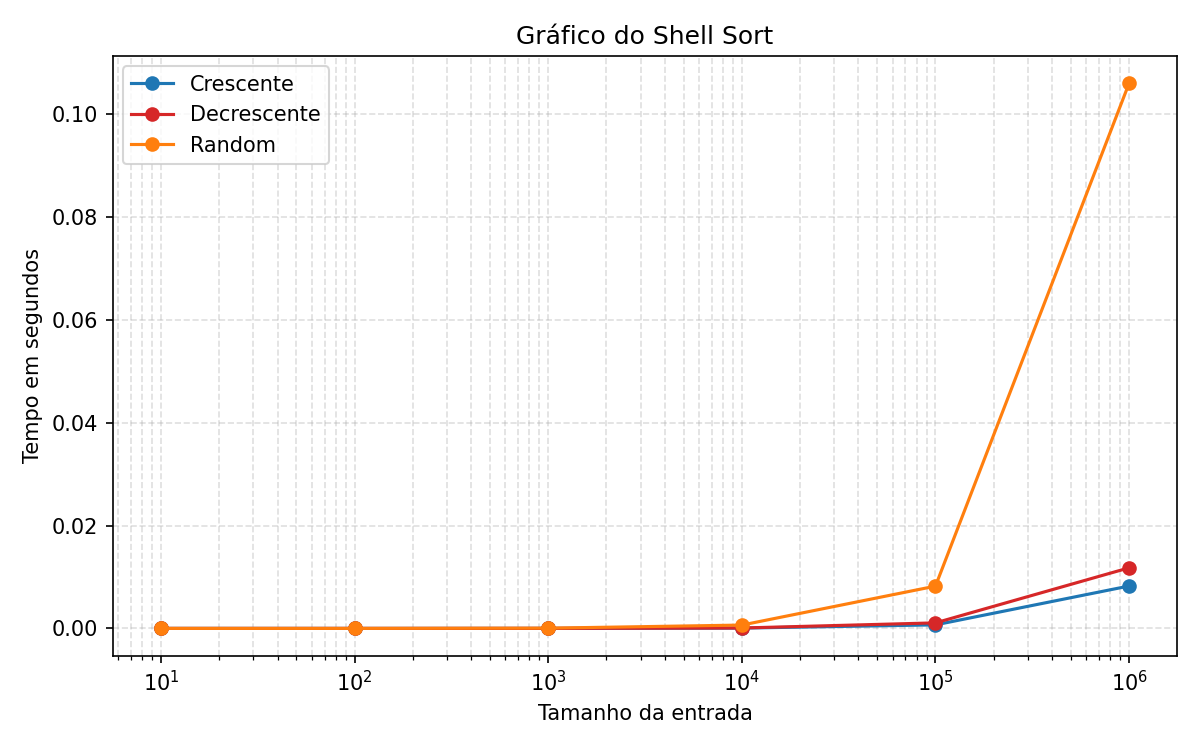
\includegraphics[width=14cm]{Imagens/Shell Sort/grafico.png}
    \caption{Gráfico de tempo por tamanho do algoritmo Shell Sort (escala linear)}
    \label{fig:grafico_shell}
\end{figure}

O Gráfico \ref{fig:grafico_shell_log} em escala logarítmica evidencia que mesmo a entrada randômica, a mais lenta das três para este algoritmo, é ordens de grandeza mais rápida do que qualquer um dos três algoritmos anteriores ($O(n^2)$) para o mesmo tamanho de instância: para 1.000.000 de elementos randômicos, cerca de 760 vezes mais rápida que o Insertion Sort e cerca de 8.800 vezes mais rápida que o Selection e o Bubble Sort. Ao aumentar o tamanho de 100.000 para 1.000.000 de elementos (10 vezes), o tempo foi multiplicado por 12,0 (crescente), 10,9 (decrescente) e 12,9 (randômica), valores próximos do fator 12,0 esperado para $n \log n$ e muito abaixo do fator 100 de um crescimento quadrático. Essa é a principal conclusão prática deste capítulo, retomada na Tabela de Comparação e no Gráfico Geral ao final deste trabalho, onde o Shell Sort também é comparado com o Merge Sort.

\begin{figure}[htbp]
    \centering
    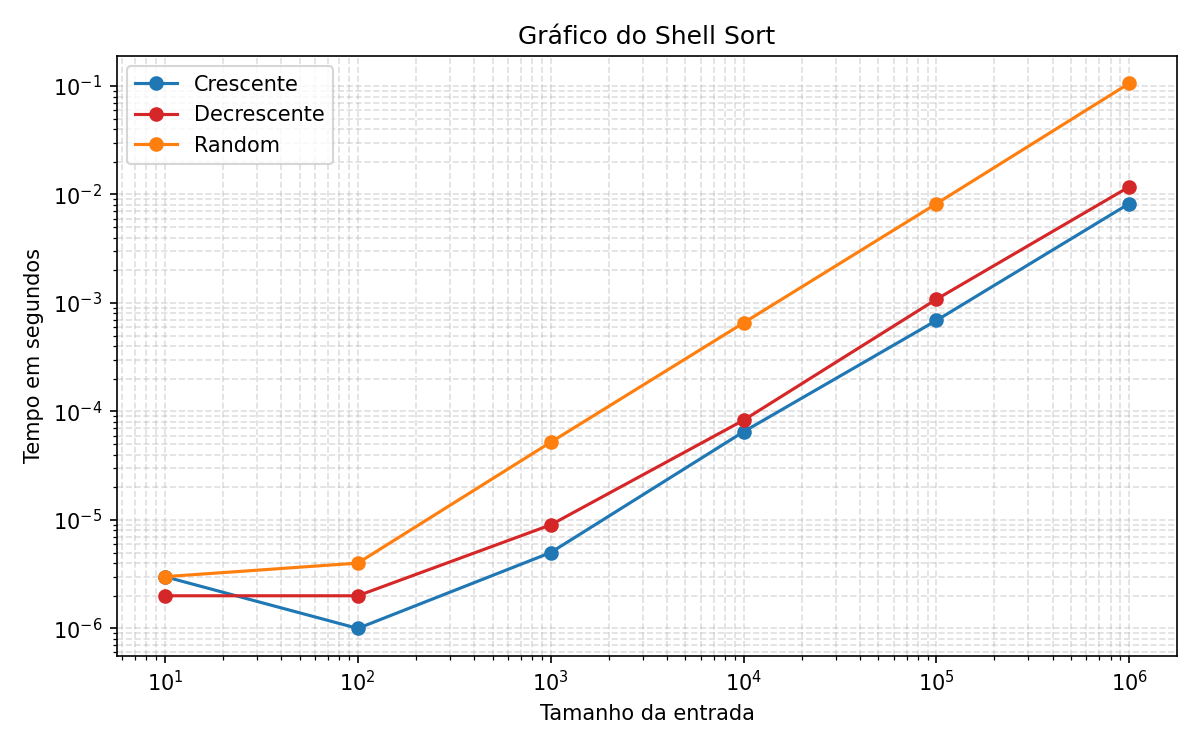
\includegraphics[width=14cm]{Imagens/Shell Sort/grafico_log.png}
    \caption{Gráfico de tempo por tamanho do algoritmo Shell Sort (escala logarítmica)}
    \label{fig:grafico_shell_log}
\end{figure}
